\section{Script, Source Corpus and the One Collapse}
\label{sec:results-interventions}

The diagnosis so far took each model's scores as given. Two interventions now ask what moves them while holding the
target items fixed: the first changes only the script in which the target comments are written, the second changes
the corpus on which the model was trained.

\subsection{The same comments in another script}
\label{sec:results-script}

Code-mixed Chaos comes in Banglish and in a row-aligned Bangla-script rendition of the same comments with identical
labels. The release describes this rendition as a transliteration and also as a translation, so the comparison holds
the comments and labels fixed but may change some wording along with the script. Moving the comments into Bangla
script raises encoder AUROC by 0.212--0.225 for IndicBERT (four training variants), 0.159 for mDeBERTa-v3,
0.071--0.096 for XLM-R-base, 0.043 for MuRIL and 0.022--0.036 for BanglaBERT, while the zero-shot language models
change by $-0.001$ to $+0.055$ (Figure~\ref{fig:script}). Script coverage thus explains part of the encoders'
difficulty with romanised text, and most for the models whose pretraining saw least of it. It also moves the
threshold: the BD-SHS encoders label 16.4\% of the Banglish comments as toxic and 26.1\% of the same comments in Bangla
script, against 50\% in the gold labels, so even with the script restored the predicted proportions remain far from
the target's. Script coverage does not explain the OffMix-3L collapse: MuRIL, which was pretrained with
transliterated text, still ranks OffMix-3L at 0.546.

\begin{figure}[t]
\centering
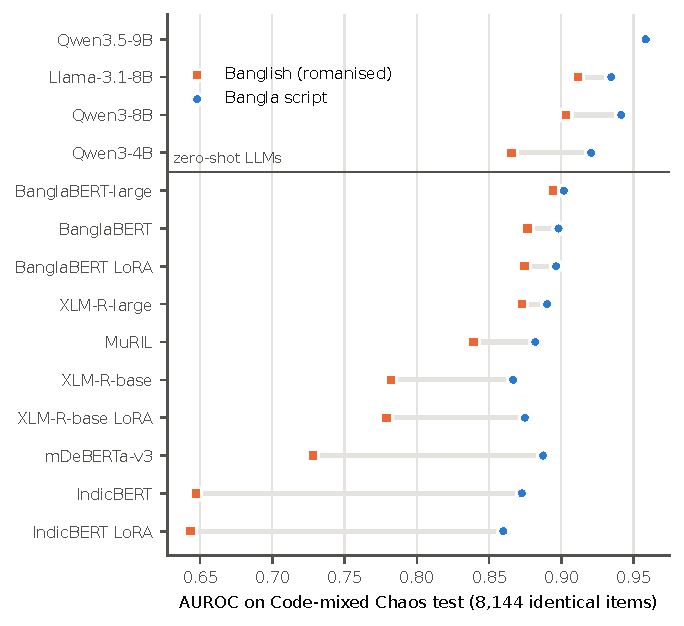
\includegraphics[width=\linewidth]{script_intervention_auroc.pdf}
\Description{Dot plot of AUROC for each encoder configuration and language model on the same comments in Banglish and in Bangla script; encoders gain up to about 0.2 from the Bangla script, language models change little.}
\caption{The same Code-mixed Chaos test comments in Banglish and in Bangla script: AUROC of every BD-SHS-trained
encoder configuration (mean over converged runs) and of each zero-shot language model, after each system's source
TS.}
\label{fig:script}
\end{figure}

\subsection{Changing the source corpus: a definition-by-language factorial}
\label{sec:results-factorial}

BD-SHS annotates hate speech \citep{romim2022bdshs}. OffMix-3L shares the label set of OLID, whose guidelines count
any unacceptable language as offensive, including untargeted profanity \citep{zampieri2019olid}, and its authors
build their synthetic training data from English corpora with those labels \citep{goswami2023offmix}. Training the
same three architectures on English OLID instead of BD-SHS raises OffMix-3L AUROC from 0.519 to 0.819, but this
comparison changes the training corpus, its label definition and its language at once. The factorial separates the
language. Cells A and B are the untranslated sources (BD-SHS in Bangla, OLID in English); C is OLID translated into
Bangla and D is BD-SHS translated into English; E and F are round trips that bring each corpus back to its own language
through the other one. Within each language two machine-translated cells then differ in their source corpus (E
against D in English, C against F in Bangla), and also in the number of translation passes (two for E and F, one for C
and D); the main effect over the four translated cells balances the passes.

\begin{figure}[t]
\centering
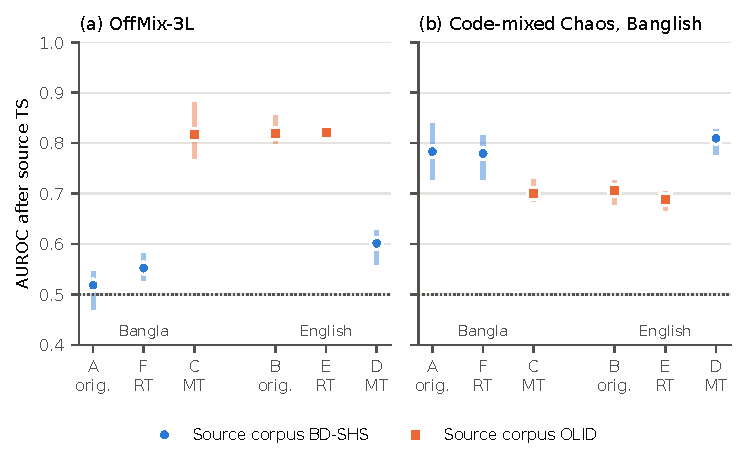
\includegraphics[width=\linewidth]{source_corpus_factorial.pdf}
\Description{Two panels of AUROC for six training cells; on OffMix-3L the OLID-based cells rank near 0.82 and the BD-SHS-based cells between 0.52 and 0.60, while on Banglish the order reverses.}
\caption{AUROC of the six factorial cells after source TS: XLM-R-base, MuRIL and mDeBERTa-v3 trained on each source
(points: mean over the 15 runs; bars: range of the three architecture means). Bangla cells: A, BD-SHS; F, BD-SHS after
a round trip through English; C, OLID translated into Bangla. English cells: B, OLID; E, OLID after a round trip
through Bangla; D, BD-SHS translated into English. orig.: untranslated; MT: translated; RT: round trip.}
\label{fig:factorial}
\end{figure}

The family of four contrasts on OffMix-3L AUROC was fixed in the public repository before cells C to F were trained
but after A and B were known, so it is pre-specified for the translated cells rather than for the whole experiment. All four favour the OLID corpus (Figure~\ref{fig:factorial}): $+0.220$ in English (E minus D, 95\%
interval 0.175--0.267), $+0.264$ in Bangla (C minus F, 0.207--0.316), $+0.242$ for the main effect over the four
translated cells (0.205--0.278), and $+0.343$ for its difference-in-differences against Banglish Chaos (0.311--0.375),
each with a Holm-adjusted stratified permutation $p < 0.001$ over 15 runs per cell. The language of the translated
training data matters far less: the language main effect on OffMix-3L is $-0.027$ (interval $-0.059$ to $0.006$,
$p = 0.132$). Within five writing-style clusters of OffMix-3L, which absorb much of its artifacts, the source-corpus
effect remains ($+0.209$ in English and $+0.244$ in Bangla).

The same contrast does not generalise. On natural Banglish the source-corpus main effect reverses to $-0.101$
(interval $-0.112$ to $-0.089$), on the BD-SHS test set it is $-0.129$, and on the OLID test set $+0.101$: each corpus
ranks its own kind of text best, and on MixTox-SA the effect is $-0.005$ ($p = 0.431$). The factor that the factorial
manipulates is therefore the source corpus together with its translation pipeline, that is, its label definition,
annotators and sampling of text as they survive machine translation, rather than the definition alone, and the inference covers the variation over seeds and architectures given one
translation, one MT system and one target. Translation also removes offensive words more than other words: over a
round trip, OLID keeps 0.680 of the offensive-associated words of offensive items (95\% interval 0.625--0.733) against
0.817 for frequency-matched control words, and BD-SHS keeps 0.249 against 0.294. This word-level sanitisation is a
limitation of the translated cells, but it cannot produce the OffMix-3L result, since the OLID-based cells that lost
those words still rank OffMix-3L at 0.816 and 0.822. We read the OffMix-3L collapse as a mismatch between the BD-SHS
corpus and that target, a property of a student-written stress case rather than of code-mixing; the natural
code-mixed targets, on which BD-SHS models keep their ranking, carry the general claims. Matching the corpus restores
the ranking but not the threshold: the OLID-trained models label 8.4\% of OffMix-3L as offensive, against 47.8\% in the
gold labels, which is the threshold shift of Section~\ref{sec:results-diagnosis} again.
